\documentclass[ignorenonframetext,]{beamer}
\usetheme{Darmstadt}
\usecolortheme{beaver}
\usefonttheme{structurebold}
\usenavigationsymbolstemplate{}
\setbeamertemplate{caption}[numbered]
\setbeamertemplate{caption label separator}{:}
\setbeamercolor{caption name}{fg=normal text.fg}
\usepackage{amssymb,amsmath}
\usepackage{ifxetex,ifluatex}
\usepackage{fixltx2e} % provides \textsubscript
\usepackage{lmodern}
\usepackage{subfig}
\ifxetex
\usepackage{fontspec,xltxtra,xunicode}
\defaultfontfeatures{Mapping=tex-text,Scale=MatchLowercase}
\newcommand{\euro}{€}
\else
\ifluatex
\usepackage{fontspec}
\defaultfontfeatures{Mapping=tex-text,Scale=MatchLowercase}
\newcommand{\euro}{€}
\else
\usepackage[T1]{fontenc}
\usepackage[utf8]{inputenc}
\fi
\fi
% use upquote if available, for straight quotes in verbatim environments
\IfFileExists{upquote.sty}{\usepackage{upquote}}{}
% use microtype if available
\IfFileExists{microtype.sty}{\usepackage{microtype}}{}
\usepackage{longtable,booktabs}
\usepackage{caption}
% These lines are needed to make table captions work with longtable:
\makeatletter
\def\fnum@table{\tablename~\thetable}
\makeatother
\usepackage{graphicx}
\makeatletter
\def\maxwidth{\ifdim\Gin@nat@width>\linewidth\linewidth\else\Gin@nat@width\fi}
\def\maxheight{\ifdim\Gin@nat@height>\textheight0.8\textheight\else\Gin@nat@height\fi}
\makeatother
% Scale images if necessary, so that they will not overflow the page
% margins by default, and it is still possible to overwrite the defaults
% using explicit options in \includegraphics[width, height, ...]{}
\setkeys{Gin}{width=\maxwidth,height=\maxheight,keepaspectratio}



\setlength{\parindent}{0pt}
\setlength{\parskip}{6pt plus 2pt minus 1pt}
\setlength{\emergencystretch}{3em}  % prevent overfull lines
\setcounter{secnumdepth}{0}

\title{Advanced Research Tools for Economics and Business Administration}
\author{Thomas de Graaff}
\date{January 15, 2016}

\begin{document}
	\frame{\titlepage}

\section{Introduction}\label{introduction}

\subsection{Introduction}\label{introduction-1}

\begin{frame}{Why this workshop?}

\begin{itemize}
\item
  In the \emph{social sciences} few attention to what tools to use (and
  why they make sense)
\item
  \LaTeX is used very much in the scientific world and can \emph{work}
  together with

  \begin{itemize}
  \itemsep1pt\parskip0pt\parsep0pt
  \item
    Stata/R
  \item
    Markdown/HTML
  \item
    Reference managers
  \end{itemize}
\item
  Why \emph{I} want to give this workshop

  \begin{itemize}
  \itemsep1pt\parskip0pt\parsep0pt
  \item
    intrinsic interest
  \item
    my goal: pre-conferences workshops / courses
  \end{itemize}
\end{itemize}

\end{frame}

\begin{frame}{What I want (and don't want) with this workshop}

\begin{itemize}
\item
  Give a general introduction of why some tools work together

  \begin{itemize}
  \itemsep1pt\parskip0pt\parsep0pt
  \item
    Why \LaTeX
  \item
    Why reference managers
  \end{itemize}
\item
  Give an introduction to \LaTeX

  \begin{itemize}
  \itemsep1pt\parskip0pt\parsep0pt
  \item
    First the basics
  \item
    Next workshop: some advanced stuff
  \end{itemize}
\item
  What \emph{I} do not want

  \begin{itemize}
  \itemsep1pt\parskip0pt\parsep0pt
  \item
    Tell you what applications to use (\textbf{you} need to decide and
    make a \textbf{well-informed} decision)
  \end{itemize}
\end{itemize}

\end{frame}

\section{\LaTeX}\label{section}

\subsection{Introduction}\label{introduction-2}

\begin{frame}{Background}

\begin{itemize}
\item
  \TeX has been devised by Donald E. Knuth in the late 70's
\item
  \LaTeX is a set of macro's around TeX and devised in the 80's
\item
  \LaTeX is a \emph{typesetting program}, not a \emph{Word processor}

  \begin{itemize}
  \itemsep1pt\parskip0pt\parsep0pt
  \item
    It is actually some code that needs to be compiled
  \item
    Code is typed in by an editor
  \end{itemize}
\item
  So, huge differences between

  \begin{itemize}
  \item
    Word processor: Open Office, Word
  \item
    Typesetter: \LaTeX, Adobe's InDesign (in general XML)
  \item
    Editors:

    \begin{itemize}
    \itemsep1pt\parskip0pt\parsep0pt
    \item
      Specific editors: TexStudio, TexShop, RStudio
    \item
      General editors: Sublime, TextMate, Notepad++, Vim, Emacs
    \end{itemize}
  \end{itemize}
\end{itemize}

\end{frame}

\subsection{Why \LaTeX}\label{why}

\begin{frame}{Disadvantages}

\begin{itemize}
\item
  Not WYSIWYG
\item
  You nead to learn (quite) some commands

  \begin{itemize}
  \itemsep1pt\parskip0pt\parsep0pt
  \item
    Learning curve, but
  \item
    hurray for
    \href{https://wch.github.io/latexsheet/latexsheet.pdf}{cheat sheets}
    and Google
  \end{itemize}
\item
  Difficult to cooperate with people that went to the \emph{dark side}
\item
  \emph{Basic} \LaTeX has \emph{difficulties} with incorporating new
  fonts (Hoefler, minion pro)

  \begin{itemize}
  \itemsep1pt\parskip0pt\parsep0pt
  \item
    XeTeX
  \item
    For the purists: \LaTeX~does it right
    \href{http://oestrem.com/thingstwice/2007/05/latex-vs-word-vs-writer/}{(\LaTeX vs
    Word)}
  \end{itemize}
\end{itemize}

\end{frame}

\begin{frame}{Advantages}

\begin{itemize}
\itemsep1pt\parskip0pt\parsep0pt
\item
  Free (as in beer) and ubiquitous
\item
  WYSIWYM
\item
  Consistent lay-out throughout the whole document (including tables,
  appendices, formulas, source code, etc)
\item
  Internal references are a breeze (references, tables of\ldots{},
  indices)
\item
  Forced to structure documents
\item
  Macros, thus scriptable
\item
  Large community, thus a package for almost everything (books,
  articles, presentation, posters, exams, musicscores)
\item
  Superior typography \& output
\item
  Large publishers (i.e., Elsevier and Springer) have \LaTeX~templates
  for their articles
\end{itemize}

\end{frame}

\subsection{Technicalities}\label{technicalities}

\begin{frame}{How does it work in practice?}

\begin{itemize}
\item
  You edit a \texttt{.tex} file without thinking about how it looks

  \begin{itemize}
  \itemsep1pt\parskip0pt\parsep0pt
  \item
    distraction free writing (yeah right)
  \end{itemize}
\item
  You then compile it

  \begin{itemize}
  \itemsep1pt\parskip0pt\parsep0pt
  \item
    \LaTeX is unforgiving: if there is an error, usually it does not
    compile
  \item
    Typically, errors are missing brackets or parentheses.
  \end{itemize}
\item
  Typically, source \texttt{.tex} file is compiled into \texttt{.pdf}
\end{itemize}

\end{frame}

\begin{frame}{A process diagram}
\centering
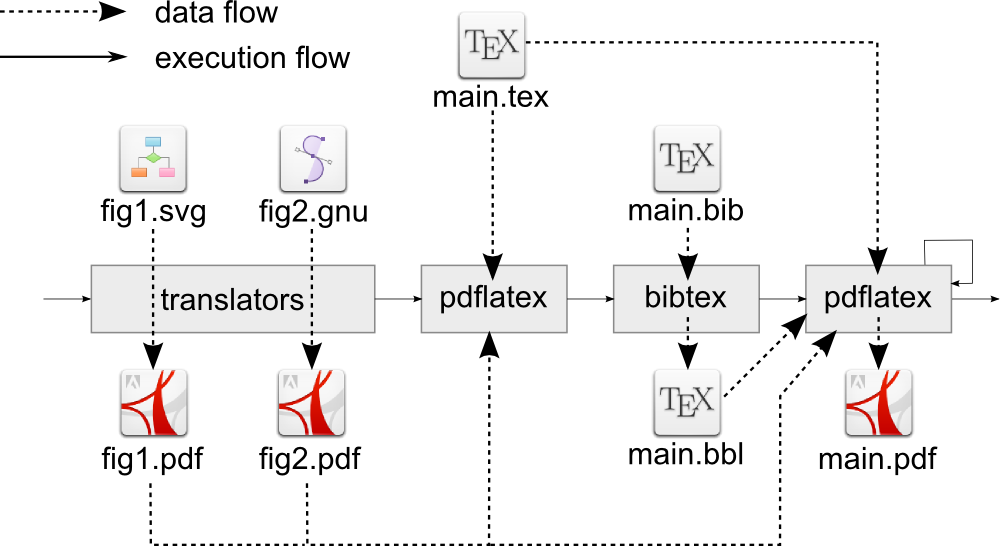
\includegraphics{fig/process.png}

\end{frame}

\section{Workflow: a bigger picture}\label{workflow-a-bigger-picture}

\subsection{Why bother?}\label{why-bother}

\begin{frame}{Why bother about workflow or tools?}

\begin{itemize}
\item
  Good scientific practice: \emph{document how you have achieved your
  results}; this ensures

  \begin{itemize}
  \itemsep1pt\parskip0pt\parsep0pt
  \item
    Reproducibility
  \item
    Transparency
  \item
    Modularity
  \item
    Portability (across systems and users)
  \item
    Efficiency
  \item
    Self-sanity
  \end{itemize}
\end{itemize}

\end{frame}

\begin{frame}{When should I adopt new tools/workflow?}

\begin{itemize}
\itemsep1pt\parskip0pt\parsep0pt
\item
  The sooner the better (you really have time now)
\item
  But think twice about which one (switching is costly; not in terms of
  beer but in terms of time)
\item
  Start one step at a time (starting with \LaTeX is a pretty neat idea)
\end{itemize}

\emph{A journey of a thousand miles begins with a single step}

Lao-tzu

\end{frame}

\begin{frame}{In general}

\begin{quote}
In science consensus is irrelevant. What is relevant is reproducible
results. The greatest scientists in history are great precisely because
they broke with the consensus (Michael Crichton)
\end{quote}

\end{frame}

\begin{frame}{In data science}

\begin{itemize}
\item
  Typically, a publication is not at the heart of research

  \begin{itemize}
  \itemsep1pt\parskip0pt\parsep0pt
  \item
    Code
  \item
    Data
  \end{itemize}
\end{itemize}

\begin{quote}
The data and code used to make a finding are available and they are
sufficient for an independent researcher to recreate the finding (Peng,
2011)
\end{quote}

\end{frame}

\begin{frame}{Code, documentation and output}

\begin{enumerate}
\def\labelenumi{\arabic{enumi}.}
\item
  Synonyms
\item
  All based on \texttt{.txt} files
\item
  Encompasses almost anything

  \begin{itemize}
  \itemsep1pt\parskip0pt\parsep0pt
  \item
    data itself (\texttt{.csv}, \texttt{.txt})
  \item
    set of commands for data cleaning and statistical analysis
    (\texttt{.do}, \texttt{.R})
  \item
    database with references (\texttt{.bib})
  \item
    text for articles, presentations or websites (\texttt{.tex},
    \texttt{.html})
  \end{itemize}
\item
  Only output is displayed/interpreted differently (e.g., in a browser
  or pdf viewer)
\end{enumerate}

\end{frame}

\subsection{Folder structure and file
names}\label{folder-structure-and-file-names}

\begin{frame}{Folder structure of your new project (theses, paper,
research)}

\begin{itemize}
\item
  Think \emph{a priori} about project set-up

  \begin{itemize}
  \itemsep1pt\parskip0pt\parsep0pt
  \item
    Seperate analysis, data and output files
  \end{itemize}
\item
  Be careful with source data!

  \begin{itemize}
  \item
    Seperate source and derived data files
  \item
    Typically

    \begin{itemize}
    \itemsep1pt\parskip0pt\parsep0pt
    \item
      you get/collect data
    \item
      transform data
    \item
      analyse data
    \end{itemize}
  \item
    Keep track of all these stages!
  \end{itemize}
\end{itemize}

\end{frame}

\begin{frame}{Why is version control systems such a neat idea}


\includegraphics{fig/phdcomic.png}

\end{frame}

\section{Reference managers}\label{reference-managers}

\subsection{Why?}\label{why-1}

\begin{frame}{Why reference managers?}

This is a life saver!

\begin{quote}
Use one!
\end{quote}

Several applications out there:

\begin{itemize}
\itemsep1pt\parskip0pt\parsep0pt
\item
  In this case Mendeley (free but not open source)
\item
  Make sure it exports to \texttt{.bib} files
\item
  Search for references (google scholar, jstor, etc.)
\item
  Mendeley can import \texttt{.pdf}'s
\end{itemize}

\end{frame}

\section{\LaTeX~lab}\label{lab}

\subsection{The basics}\label{the-basics}

\begin{frame}{Installation}

\begin{enumerate}
\def\labelenumi{\arabic{enumi}.}
\itemsep1pt\parskip0pt\parsep0pt
\item
  First, install \LaTeX~

  \begin{itemize}
  \itemsep1pt\parskip0pt\parsep0pt
  \item
    in default location
  \end{itemize}
\item
  Install, TeXstudio

  \begin{itemize}
  \itemsep1pt\parskip0pt\parsep0pt
  \item
    Which can then automatically find \LaTeX\\
  \end{itemize}
\end{enumerate}

\end{frame}

\begin{frame}[fragile]{Basic set-up of a \LaTeX~file}

\begin{verbatim}
\documentclass[]{article}
%opening
\title{}
\author{}

\begin{document}

\maketitle

\begin{abstract}
\end{abstract}

\section{}

\end{document}
\end{verbatim}

\end{frame}

\begin{frame}[fragile]{Assignment 1}

Create an abstract, title, authors, date, table of contents and create a
section and some subsections:

\begin{itemize}
	\item Give a date: \texttt{\textbackslash{}date\{\}}
	\item Create subsections: \texttt{\textbackslash{}section\{\}}, \texttt{\textbackslash{}subsection\{\}}, \texttt{\textbackslash{}subsubsection\{\}}, \texttt{\textbackslash{}chapter\{\}}
	\item Insert a table of contents: \texttt{\textbackslash{}tableofcontents\{\}}
\end{itemize}

\end{frame}

\begin{frame}[fragile]{Further text control}

\begin{itemize}
\item
  itemization

\begin{verbatim}
\begin{itemize}
\item bla bla bla
\end{itemize}
\end{verbatim}
\item
  enumeration

\begin{verbatim}
\begin{enumerate}
\item bla bla bla
\end{enumerate}
\end{verbatim}
\item
  bold: \texttt{\textbackslash{}textbf\{\}}
\item
  emphasize: \texttt{\textbackslash{}textit\{\}} or
  \texttt{\textbackslash{}emph\{\}}
\end{itemize}

\end{frame}

\begin{frame}[fragile]{Inserting equations}

\begin{itemize}
\item
  Inline: \$e=mc\^{}2\$ will be \(e=mc^2\) or

\begin{verbatim}
\begin{equation}
e=mc^2
\end{equation}
\end{verbatim}

  will render in

  \begin{equation}
  e=mc^2
  \end{equation}
\item
  Equations can be as complex (cool) as you want
\item
  \href{http://estudijas.lu.lv/pluginfile.php/14809/mod_page/content/16/instrukcijas/matematika_moodle/LaTeX_Symbols.pdf}{Cheat
  sheet mathematics:}
\end{itemize}

\end{frame}

\begin{frame}{Assignment 2:}

Produce the well-known univariate regression formula: \[
y_i = \alpha + \beta x_i + \epsilon_i
\]

\end{frame}

\begin{frame}{Referencing}

\begin{itemize}
\itemsep1pt\parskip0pt\parsep0pt
\item
  Internally:

  \begin{itemize}
  \itemsep1pt\parskip0pt\parsep0pt
  \item
    \texttt{\textbackslash{}label\{\}}, \texttt{\textbackslash{}ref\{\}}
  \end{itemize}
\item
  footnotes (different symbol in title)

  \begin{itemize}
  \itemsep1pt\parskip0pt\parsep0pt
  \item
    \texttt{\textbackslash{}footnote\{\}}
  \end{itemize}
\item
  literature:

  \begin{itemize}
  \itemsep1pt\parskip0pt\parsep0pt
  \item
    \texttt{cite\{\}}
  \end{itemize}
\item
  Bibliography:

  \begin{itemize}
  \itemsep1pt\parskip0pt\parsep0pt
  \item
    \texttt{\textbackslash{}bibliography\{database1\}}
  \item
    for style: \texttt{\textbackslash{}bibliographystyle\{\}}
  \end{itemize}
\end{itemize}

\end{frame}

\begin{frame}{Finally}

\begin{itemize}
\item
  Several spaces of new lines are treated as one space or new line
\item
  Some characters can not be used directly but with
  \texttt{\textbackslash{}} in front:

  \begin{itemize}
  \itemsep1pt\parskip0pt\parsep0pt
  \item
    not: \texttt{\#} \texttt{\$} \texttt{\%} \texttt{\^{}} \texttt{\&}
    \texttt{\_} \texttt{\{} \texttt{\}} \texttt{\textasciitilde{}}
    \texttt{\textbackslash{}}
  \item
    but: \texttt{\textbackslash{}\#} \texttt{\textbackslash{}\$}
    \texttt{\textbackslash{}\%} \texttt{\textbackslash{}\^{}}
    \texttt{\textbackslash{}\&} \texttt{\textbackslash{}\_}
    \texttt{\textbackslash{}\{} \texttt{\textbackslash{}\}}
    \texttt{\textbackslash{}\textasciitilde{}}
    \texttt{\textbackslash{}\textbackslash{}}
  \end{itemize}
\item
  Commands always start with \texttt{\textbackslash{}}
\item
  Comments start with \texttt{\%}
\end{itemize}

\end{frame}

\section{Next time}\label{next-time}

\subsection{Next workshop}\label{next-workshop}

\begin{frame}{What are we going to do next time?}

\begin{itemize}
\itemsep1pt\parskip0pt\parsep0pt
\item
  Use of packages
\item
  Figures
\item
  Tables
\item
  Automating \texttt{do} file outputs
\item
  Slides
\end{itemize}

\end{frame}

\end{document}
